\section{Special Features}
\label{sec:fea}%
\index{environments}\index{special features}
\index{special considerations}\html{\\}\noindent
This {section} describes major features available for processing
documents using \latextohtml.
Firstly the means whereby \latextohtml{} can be configured to produce output 
for the \htmlref{different versions}{versions} of \texttt{HTML} 
is discussed\latex{ in Section~\ref{versions}}.
Following this is a description\latex{, in Section~\ref{internat},}
of how to \htmlref{use languages}{internat} other than English. 
The options available with the \htmlref{creation and reuse of images}{imgcon},
are presented\latex{ in Section~\ref{imgcon}},
for those situations where a textual representation is inadequate or undesirable.

There are several strategies available for the \htmlref{presentation
of mathematics}{maths} according to the desired version of \texttt{HTML}. 
These are discussed in some detail\latex{, in Section~\ref{maths}}. 
Environments such as \env{figure}, \env{table}, \env{tabular}
and \env{minipage} have \htmlref{special features}{sec:figs}%
\latex{ which are discussed in Section~\ref{sec:figs}}. 
Other supported packages are \hyperref{listed}{listed in Table~}{}{styles}.


\subsection{Variation with HTML Versions\label{versions}}%
%\section{Variation with HTML Versions\label{versions}}%
\index{HTML@\texttt{HTML}!an evolving standard}%
\index{HTML@\texttt{HTML}!basic version, 2.0 }%
\index{HTML@\texttt{HTML}!current version, 3.2 }%
\index{HTML@\texttt{HTML}!future version, 4.0 }%
\html{\\}\noindent
The Hypertext Mark-up Language (\texttt{HTML}) is an evolving standard,
with different versions supporting different features.  
In order to make your documents viewable by the widest possible audience,
you should use the most advanced \texttt{HTML} version with widely-accepted usage.

\index{iso-latin1@ISO--Latin--1|see{\htmlref{character set}{IIIcharset}}}%
\index{iso-8879@ISO--8879|see{\htmlref{character set}{IIIcharset}}}%
\index{character set!ISO-8879@ISO--8879 (ISO--Latin--1)}%
\index{HTML@\texttt{HTML}!interactive forms}%
\index{HTML@\texttt{HTML}!image-maps}%

\medskip\noindent
Sometimes it is known that the audience, for which a specific document 
is intended, has limited browser capabilities. 
Or perhaps special extended capabilities are known to be available.
The \latextohtml{} translation may be customised to suit the
available functionality.

\medskip\noindent
Other \texttt{HTML} versions and extensions 
supported by \latextohtml\ are described below.
See the description of the \Cs{html\_version} command-line
\hyperref[page]{option switch}{option switch, on page~}{}{cs_htmlversion}.
%
\begin{htmllist}\htmlitemmark{RedBall}
%begin{latexonly}
\addtolength{\leftskip}{15pt}
%end{latexonly}
\index{HTML@\texttt{HTML}!Version 2.0}%
\item[Version 2.0\label{html20}]
This provides only the functionality of the \texttt{HTML} 2.0 standard.
There is little provision for aligning headings, paragraphs or images
nor for super/sub-scripts to be generated. Images are created for tables 
and other environments that use \HTMLtag{TABLE} tags with \HTMLiii;
e.g. \env{eqnarray} and \env{equation} with equation numbering.

\index{HTML@\texttt{HTML}!Version 2.1, now `i18n' extension}%
\index{Unicode|see{\htmlref{character set}{IIIcharset}}}%
\index{iso-10646@ISO--10646!Unicode}%
\index{iso-10646@ISO--10646!|see{\htmlref{character set}{IIIcharset}}}%
\index{iso-10646@ISO--10646!bidirectional languages}%
\index{character set!ISO-10646@ISO--10646 (Unicode)}%
\index{iso-8859-1@ISO--8859--1!no longer used}%
\item[i18n (internationalised fonts) \strikeout{Version 2.1}]
This extension (formerly known as \texttt{HTML} version 2.1)
provides extensions for \htmlref{internationalisation}{internat}.
Most importantly, the default character set is no longer ISO--8859--1 
but {ISO--10646} (Unicode).
This is a 16-bit character set and can thus display a much larger set of characters.
There are also provisions for bidirectional languages 
(e.g. in Arabic the text is written from right to left, 
but numerals from left to right), and provisions in \texttt{HTML} 
to determine the character set and the language used.

Not all of the symbols are available in \TeX, \latextohtml, 
or any browser yet available.  
However the `\texttt{i18n}' extension to \latextohtml\ is in preparation
for when such browsers do become available, and such characters
will be required in Web-accessible documents. 


\index{HTML@\texttt{HTML}!Version 3.0, \texttt{HTML-Math} model}%
\index{HTML@\texttt{HTML}!Version 3.1, now `math' extension}%
\index{Arena@\textsl{Arena}!math mark-up}\index{CERN!Arena@\textsl{Arena}}%
\index{browser!Arena@\textsl{Arena}}%
\item[math (\texttt{HTML3} model) \strikeout{Version 3.1}]
This extension (formerly referred to as \texttt{HTML} version 3.1)
adds support for the \htmladdnormallink{\texttt{HTML-Math} model}%
{http://www.w3.org/MarkUp/html3/maths.html}, originally
part of the proposed \texttt{HTML} 3.0 standard, see \htmlref{above}{html30}.
The only available browser
which can display this mark-up is \appl{Arena}.
Originally developed by the \htmladdnormallink{World Wide Web Consortium}%
{http://www.w3.org/Arena} as a test-bed browser,
it is no longer supported by them.

\index{mathematics!MathML}
There has been a recent proposal for a Mathematical Markup Language
(\htmladdnormallink{\texttt{MathML}}%
{http://www.w3.org/pub/WWW/TR/WD-math-970515}) 
from the W3C \htmladdnormallink{Math Working Group}%
{http://www.w3.org/pub/WWW/Markup/Math/}. 
This would suggest that the \texttt{HTML-Math} model is unlikely 
ever to be adopted; better things being expected in the near future
using \texttt{MathML}.

See also \hyperref{another page}{Section~}{}{maths} for a discussion
the the mechanisms available with \latextohtml{} for handling
mathematical equations and expressions.
\end{htmllist}




\subsection{Internationalisation\label{internat}}%
%\section{Internationalisation\label{internat}}%
\index{languages}\index{extensions!languages}\html{\\}%
A special variable \fn{\$LANGUAGE\_TITLES} 
in the initialisation or configuration files determines the language 
in which some section titles will appear. For example setting it to 
\begin{quote}
\begin{verbatim}
$LANGUAGE_TITLES = 'french';
\end{verbatim}
\end{quote}
will cause \latextohtml{} to produce ``Table des mati{\`e}res'' instead of
``Table of Contents''.
Furthermore, the value of the \Lc{today} command is presented in a format
customary in that language.

\index{languages!french}\index{languages!english}\index{languages!german}%
\index{languages!spanish}\index{languages!finnsh}%\index{languages!slovene}%
\html{\\}%
Languages currently supported are 
\env{finnish}, \env{french}, \env{english}, \env{german}
 and \env{spanish}.
It is trivial to add support for another language by creating a file
in the \fn{styles/} subdirectory, 
or by adding to the file \fn{latex2html.config}.
As a guide, here is the entry for French titles:
%begin{latexonly}
\begin{small}
%end{latexonly}
\begin{verbatim}
sub french_titles {
    $toc_title = "Table des mati\\`eres";
    $lof_title = "Liste des figures";
    $lot_title = "Liste des tableaux";
    $idx_title = "Index";
    $ref_title = "R\\'ef\\'erences";
    $bib_title = "R\\'ef\\'erences";
    $abs_title = "R\\'esum\\'e";
    $app_title = "Annexe";
    $pre_title = "Pr\\'eface";
    $fig_name = "Figure";
    $tab_name = "Tableau";
    $part_name = "Partie";
    $prf_name = "Preuve";
    $child_name = "Sous-sections";
    $info_title = "\\`Apropos de ce document...";
    @Month = ('', 'janvier', "f\\'evrier", 'mars', 'avril', 'mai',
              'juin', 'juillet', "ao\\^ut", 'septembre', 'octobre',
              'novembre', "d\\'ecembre");
    $GENERIC_WORDS = "a|au|aux|mais|ou|et|donc|or|ni|car|l|la|le|les"
        . "|c|ce|ces|un|une|d|de|du|des";
}
\end{verbatim}
%begin{latexonly}
\end{small}
%end{latexonly}
Notice how the backslash needs to be doubled, when a macro is needed
(for accented characters, say).
Also, the \texttt{\$GENERIC\_WORDS} are a list of short words to be excluded
when filenames are specially requested to be created from section-headings.
In order to provide full support for another language you may also
replace the navigation buttons which come with \latextohtml{} 
(by default in English) with your own. 
As long as the new buttons have the same file-names as the old ones, 
there should not be a problem.


\subsubsection{Alternate Character Encodings\label{fontEncodings}}%
%
\index{extension!options}%
\html{\\}%
By default, \latextohtml\ assumes that input files are
Unicode encoded with UTF8, and produces Unicode UTF8 output.

\latextohtml\ can handle input files in other encodings,
indicated by including the \texttt{inputenc}
package in the source:
%
%begin{latexonly}
\begin{small}
%end{latexonly}
\begin{verbatim}
 \usepackage[latin5]{inputenc}
\end{verbatim}
%begin{latexonly}
\end{small}
%end{latexonly}
In this case, \latextohtml\ will produce output in the
same encoding, and will indicate the encoding in the HTML
headers.
The input encodings that are recognised are listed in 
\hyperref{the following table}{Table~}{}{tab_encodings}.

\begin{table}
\begin{center}
\begin{tabular}{|>{\ttfamily}lcl|}%\hline
\multicolumn{1}{c}{\textbf{extension}}
&\multicolumn{1}{c}{\textbf{notes}}
&\multicolumn{1}{c}{\textbf{encoding}}\\\hline
unicode & (default)& ISO--10646 (Unicode)\\
latin1 &  & ISO--8859--1 (ISO-Latin-1) \\
latin2 &  & ISO--8859--2 (ISO-Latin-2) \\
latin3 &  & ISO--8859--3 (ISO-Latin-3) \\
latin4 &  & ISO--8859--4 (ISO-Latin-4) \\
latin5 &  & ISO--8859--9 (ISO-Latin-5) \\
latin6 &  & ISO--8859--10 (ISO-Latin-6)\\
koi8-r &  & RFC 1489 (Russian) \\\hline
\end{tabular}
\caption{Supported Font-encodings\label{tab_encodings}}
\end{center}
\end{table}


\subsubsection{Multi-lingual documents, using Images\label{multilang}}%
%
Some multi-lingual documents can be constructed, when all the languages
can be presented using characters from a single font-encoding,
as discussed in the \hyperref{previous section}{Section~}{}{fontEncodings}.

Another way to present multiple languages within a Web document is to
create images of individual letters, words, sentences, paragraphs
or even larger portions of text, which cannot be displayed within
the chosen font-encoding.
This is a technique that is used with \IndicHTML, for presenting
traditional Indic language scripts within Web pages.
For these the \LaTeX\ source that is to be presented as an image
needs special treatment using a ``pre-processor''. 
For the special styles defined in \IndicHTML, running the preprocessor
is fully automated, so that it becomes just another step 
within the entire image-generation process.

\medskip

The technique of using images, can be used with \emph{any} font 
whose glyphs can be typeset using \TeX{} or \LaTeX. 
Using \TeX's \Lcs{font} command, a macro is defined to declare
the special font required; 
e.g. for Cyrillic characters, using the Univ. of Washington font:
%begin{latexonly}
\begin{small}
%end{latexonly}
\begin{verbatim}
 \font\wncyr = wncyr10
\end{verbatim}
%begin{latexonly}
\end{small}
%end{latexonly}

\noindent
Now use this font switch immediately surrounded by braces:
%begin{latexonly}
\begin{small}
%end{latexonly}
\begin{verbatim}
 published by {\wncyr Rus\-ski\char26\ \char23zyk}.
\end{verbatim}
%begin{latexonly}
\end{small}
%end{latexonly}
to get:
\begin{center}
 published by {\wncyr Rus\-ski\char26\ \char23zyk}.
\end{center}


\subsection{Mathematics\label{maths}}
%\section{Mathematics\label{maths}}
%
There are various different ways in which \latextohtml{} can handle
mathematical expressions and formulas:
\begin{itemize}
\item
give a textual representation (``simple'' math);
\item
make an image of the complete formula or expression;
\item
combination of textual representation and images of
sub-expressions;
\item
\texttt{SGML}-like representation built using abstract ``entities'';\\
e.g. for the \texttt{HTML-Math} model, or for \texttt{MathML}.
%
\end{itemize}
Which is the most appropriate normally depends on the context,
or importance of the mathematics within the entire document.
What \latextohtml{} will produce depends upon
\begin{enumerate}
\item 
the version of \texttt{HTML} requested;
\item
whether or not the special `\texttt{math}' \htmlref{extension}{} has been loaded;
\item
whether the \Cs{no\_math} \htmlref{command-line option}{nomath}
has been specified, or (equivalently) the \fn{\$NO\_SIMPLE\_MATH} 
\htmlref{variable}{nomath} has been set in an initialisation file.
\end{enumerate}
%
The strategies used to translate math expressions are summarised
in \hyperref{the table below}{Table~}{}{mathconv3} for \texttt{HTML} 3.0+
and \hyperref{the subsequent table}{Table~}{}{mathconv2} for \texttt{HTML} 2.0.

\begin{table}[ht]
\begin{center}
\begin{tabular}{|c|c|p{6cm}|}
\hline
\textbf{`math'} & \textbf{switch} &\textbf{\hfill strategy adopted\hfill~}\\ \hline
 not loaded & \Cs{math} & textual representation where possible,\newline
  else image of whole expressions\\ \hline
 not loaded & --- & always generates an image of the whole\newline
 expression/environment\\ \hline
 loaded & --- &
uses entities and \HTMLtag{MATH} tags; e.g. for \texttt{HTML-Math}
 (or \texttt{MathML} in future)\\ \hline
 loaded & \Cs{no\_math} & textual representation where possible,
 with~images~of sub-expressions \\ \hline
\end{tabular}
\caption{Mathematics translation strategies, 
 for \texttt{HTML} versions 3.0 and 3.2,\protect\newline
 using \protect\HTMLtag{SUP} and \protect\HTMLtag{SUB} tags
 and \protect\HTMLtag{TABLE}s}
\label{mathconv3}
\end{center}
\end{table}

The default behavior, with no command line options,
is to generate images for all math expressions, which makes
the appearance of all mathematical expressions consistent.
This is what was used when creating\latex{ the \texttt{HTML} version of} 
this manual. 
 
\bigskip
\noindent
Since the \texttt{HTML} 2.0 standard does not include
superscripts and subscripts, via the \HTMLtag{SUP} and \HTMLtag{SUB} tags,
the options are more limited. In this case creating images of sub-expressions
is not so attractive, since virtually the whole expression would
consist of images in all but the simplest of cases.

\begin{table}[hbt]
\begin{center}
\begin{tabular}{|c|c|p{6cm}|}\hline
\textbf{`math'} & \textbf{switch} &\textbf{\hfill strategy adopted\hfill~}\\ \hline
 not loaded & --- & textual representation where possible,\newline
 else image of whole expressions\\ \hline
 not loaded & \Cs{no\_math} & always generates an image of\newline
the whole expression or environment\\ \hline
 loaded & --- &
entities and \HTMLtag{MATH} tags for~\texttt{HTML-Math}\\ \hline
 loaded & \Cs{no\_math} & always generates an image of the whole\newline
 expression or environment \\ \hline
\end{tabular}
\caption{Mathematics translation strategies,
for \texttt{HTML} version 2.0\label{mathconv2}}
\end{center}
\end{table}
\medskip \htmlrule
\index{numbered equations}\index{equations!numbered}%
\index{equations!right-justified}\html{\\}%

\noindent
Here are some examples of mathematical expressions and environments 
processed by \latextohtml{} using different strategies. 
They are automatically numbered \dots 
\begin{equation}\label{eq:demo} 
 \Phi_{l+1,m,n} = \Bigl(\Phi+h\frac{\partial\Phi}{\partial x} +
 \frac{1}{2}h^2\frac{\partial^2\Phi}{\partial x^2} +
 \frac{1}{6}h^3\frac{\partial^3\Phi}{\partial x^3} + \,\ldots\,\Bigr)_{l,m,n}
\end{equation}
\dots\ with some gratuitously {\'a}c{\c c}{\"e}nted text in-between \dots
%
\index{equations!array}%
\index{eqnarray@\env{eqnarray} environment!example}%
%
\begin{eqnarray}
\frac{\Phi_{l+1,m,n}-2\Phi_{l,m,n}+\Phi_{l-1,m,n}}{h^{2}} +
\frac{\Phi_{l,m+1,n}-2\Phi_{l,m,n}+\Phi_{l,m-1,n}}{h^{2}} \nonumber \\
+ \frac{\Phi_{l,m,n+1}-2\Phi_{l,m,n}+\Phi_{l,m,n-1}}{h^{2}} = -I_{l,m,n}(v)\;.
\end{eqnarray}
The latter example uses an \env{eqnarray} environment
and the \Lc{nonumber} command to suppress
the equation number on the upper line.

The default image format is Scalable Vector Graphics (SVG),
which looks crisp at all resolutions.  If bitmap image
formats are used (PNG or GIF), various options are
available to control antialiasing and the resolution
of the images.  These options are discussed in the
following sections.

\index{image generation!using htmlimage@using \Lc{htmlimage}}

For combinations of options that do not generate images for all
math expressions, it is possible to control image generation
at the level of individual expression.
By inserting an \verb|\htmlimage{}| command into a \env{math},
\env{equation} or \env{displaymath} environment, a single image
will be created for the whole environment. For an \env{eqnarray}
environment, this will lead to having a single separate image 
for each of the aligned portions. 
The argument to \Lc{htmlimage} need not be empty, but may contain
information which is used to affect characteristics of the resulting
image. An example of how this is used is given \htmlref{below}{ex:aalias},
and a fuller discussion of the allowable options is given in
\hyperref{the next section}{Section~}{}{imgcon}.


\index{scale-factors!for math images}%
\paragraph*{Scale-factors for Mathematics.\label{mathscales}}
%
For bitmap image formats (PNG or GIF, as opposed to SVG),
the scale factor controls the image resolution.
When a bitmap image 
is made of a mathematical formula or expression,
it is generally made at a larger size 
than is normally required on a printed page.
This is to compensate for the reduced resolution of a computer screen
compared with laser-print.  
The amount of this scaling is given by the
value of a configuration variable \fn{\$MATH\_SCALE\_FACTOR},
by default set to 1 in \fn{latex2html.config}. 
A further variable \fn{\$DISP\_SCALE\_FACTOR} is used with
`displayed math' equations and formulas.
This value multiplies the \fn{\$MATH\_SCALE\_FACTOR} 
to give the actual scaling to be used.
The main purpose of this extra scaling is to allow some clarity in
super/subscripts etc.


\index{anti-aliasing!comparison}%
\paragraph*{Anti-aliased Images.\label{ex:aalias}}
\hyperref{Here are}{Figure~}{ shows}{eq:pics} the same equations
as \htmlref{previously}{eq:demo}, this time as images of the 
complete contents of the \env{equation} environment, 
and complete aligned parts of rows in an \env{eqnarray}.
\begin{latexonly}
These are images, as they would appear if the \texttt{HTML} page
were to be printed from the browser. A scaling of 60\% has been
applied to counteract the combined effects of the \fn{\$MATH\_SCALE\_FACTOR} 
of 1.4 and \fn{\$DISP\_SCALE\_FACTOR} of 1.2, 
used for the \texttt{HTML} version of this manual. 
\end{latexonly}
For a comparison, the second group of images use anti-aliasing effects, 
whereas the first image does not; a 600\,dpi printing is probably necessary
to appreciate the difference in quality. Compare these images with those in
\hyperref{a later section}{Section~}{}{printqual}.

\begin{figure}[hb]
\begin{makeimage}
\end{makeimage}
\begin{htmlonly}
\begin{equation}
\htmlimage{no_antialias}
\Phi_{l+1,m,n} = \Bigl(\Phi+h\frac{\partial\Phi}{\partial x} +
\frac{1}{2}h^2\frac{\partial^2\Phi}{\partial x^2} +
\frac{1}{6}h^3\frac{\partial^3\Phi}{\partial x^3} + \,\ldots\,\Bigr)_{l,m,n}
\end{equation}
\begin{eqnarray}
\htmlimage{}
\frac{\Phi_{l+1,m,n}-2\Phi_{l,m,n}+\Phi_{l-1,m,n}}{h^{2}} +
\frac{\Phi_{l,m+1,n}-2\Phi_{l,m,n}+\Phi_{l,m-1,n}}{h^{2}} \nonumber \\
+ \frac{\Phi_{l,m,n+1}-2\Phi_{l,m,n}+\Phi_{l,m,n-1}}{h^{2}} = -I_{l,m,n}(v)\;.
\end{eqnarray}
\end{htmlonly}
%
\begin{latexonly}
\begin{equation}
 \setbox1=\hbox{\scalebox{.6}{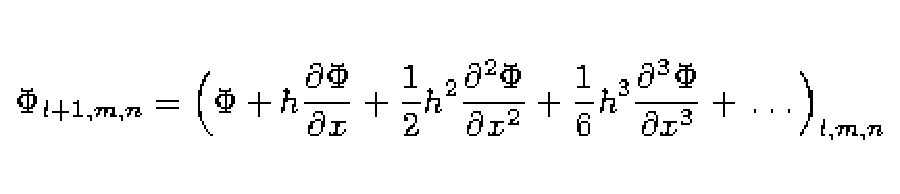
\includegraphics{psfiles/eqn1}}}
 \lower.5\ht 1\box1
\end{equation}
\begin{eqnarray}
 \nonumber
 \setbox1=\hbox{\scalebox{.6}{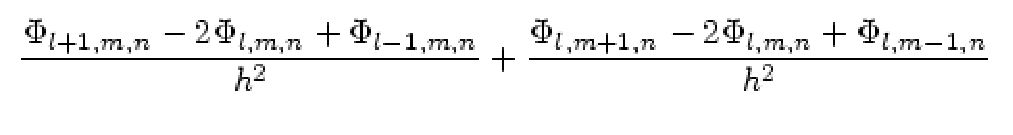
\includegraphics{psfiles/eqarrA1}}}
 \lower.5\ht1 \box1&&\\
 \setbox1=\hbox{\scalebox{.6}{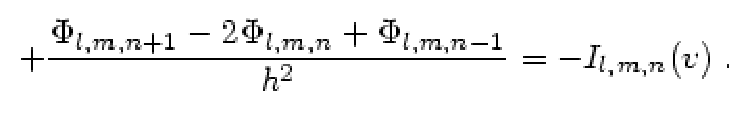
\includegraphics{psfiles/eqarrB1}}}
 \lower.5\ht1 \box1&&
\end{eqnarray}
\end{latexonly}
\caption{Images of equation displays, at normal screen resolution}\label{eq:pics}
\end{figure}

\noindent
These images of the whole environment were created 
using the \Lc{htmlimage} command, to suppress the extended parsing 
that usually occurs when the `\texttt{math}' extension is loaded; viz.
%
%begin{latexonly}
\begin{small}
%end{latexonly}
\begin{verbatim}
\begin{equation}
\htmlimage{no_antialias}
\Phi_{l+1,m,n} = \Bigl(\Phi+h\frac{\partial\Phi}{\partial x} +
...
\end{equation}
%
\begin{eqnarray}
\htmlimage{}
\frac{\Phi_{l+1,m,n}-2\Phi_{l,m,n}+\Phi_{l-1,m,n}}{h^{2}} +
...
\end{eqnarray}
\end{verbatim}
%begin{latexonly}
\end{small}
%end{latexonly}
Further aspects of the options available when generating images 
are discussed in \htmlref{the next section}{imgcon}, in particular 
with regard to the quality of \htmlref{printed images}{printqual}.



\index{mbox@\Lc{mbox} command with math!generates an image}%
\paragraph*{The \Lc{mbox} command.}
Another way to force an image to be created of a mathematical expression,
when global settings are not such as to do this anyway, 
is via the \Lc{mbox} command having math delimiters within its argument.

Normally \Lc{mbox} is used to set a piece of ordinary text within a 
mathematics environment. It is not usual to have math delimiters 
\texttt{\$...\$} or \Lc{(}...\Lc{)} within the argument of an \Lc{mbox}. 
Whereas earlier versions of \latextohtml{} simply ignored the \Lc{mbox} 
command (treating its argument as normal text), 
the presence of such delimiters now results in an image being
generated of the \emph{entire contents} of the \Lc{mbox}.
It is not necessary for there to be any actual mathematics inside
the \Lc{mbox}'s contents;\html{\\}
e.g. \verb|\mbox{...some text...${}$}|
will cause an image to be created of the given text.


\index{parbox@\Lc{parbox} command!generates an image}%
\paragraph*{The \Lc{parbox} command.}
The \Lc{parbox[}\Meta{align}\verb|]{|\Meta{width}\verb|}{|\Meta{text}\verb|}| 
command also generates an image of its contents,
except when used within a \env{tabular} environment, or other
similar table-making environment.
Here the important aspect is the width specified for the given
piece of text, and any special line-breaks or alignments that
this may imply. Hence to get the best effect, \LaTeX{} is used
to typeset the complete \Lc{parbox}, with its specified width,
alignment and contents, resulting in an image.


\index{heqn.sty@\texttt{heqn.sty} style-file}%
\index{package!heqn@\env{heqn}}\index{heqn@\env{heqn} package}%
\index{eqnarray@\env{eqnarray} environment}%
\index{equation@\env{equation} environment}\html{\\}%
\paragraph*{The \env{heqn} package.}
%
If you need \texttt{HTML} 2.0 compatible Web pages,
and have a document with a great many displayed equations, 
then you might try using the \env{heqn} package.  
Inclusion of the \fn{heqn.sty} file has absolutely
no effect on the printed version of the article, 
but it does change the way in which \latextohtml{} translates
displayed equations and equation arrays.  
It causes the equation numbers of the \env{equation}
environment to be moved outside of the images themselves, 
so that they become order-independent and hence recyclable.  
Images that result from the \env{eqnarray} environment are also recyclable,
so long as their equation numbers remain unchanged from the previous run.  

\index{nonumber@\Lc{nonumber}}%
\index{package!html@\env{html}}%
\index{html@\env{html} package}\html{\\}%
The \Lc{nonumber} command is recognised 
in each line of the equation array, to suppress the equation number.
A side-effect of this approach is that equation numbers will
appear on the left side of the page.
The \env{heqn} package requires the \env{html} package.%

\smallskip\noindent
Using \texttt{HTML} Version 3.2 the \env{heqn} package is quite redundant,
since equation numbers are placed in a separate \HTMLtag{TABLE} cell
to the mathematical expressions themselves.
It is \emph{not} required and should \emph{not} be requested, since this will
override some of the improved functionality already available.




\subsection{Figures and Image Conversion\label{imgcon}%
%\section{Figures and Image Conversion\label{imgcon}%
\index{images@images\protect\label{IIIimages}}}%
\tableofchildlinks*\htmlrule
%
\noindent
\latextohtml{} converts equations, special accents, external \PS\ 
files, and \LaTeX{}  environments it cannot directly translate into 
inlined images. This section describes how it is possible to control
the final appearance of such images. For purposes of discussion \dots
\begin{itemize}
\item
``small images'' \index{images!small images}\html{\\}%
refers to inline math expressions, special accents and
any other \LaTeX{} command which causes an image to be generated; while \dots 
\item
``figures'' \index{images!figures}\html{\\}%
applies to image-generating \LaTeX{} environments 
(e.g. \env{makeimage}, \env{figure}, \env{table} (with \texttt{HTML} 2.0), 
 and displayed math environments when required to generate images, etc.).
\end{itemize}

\index{images!math scale-factor}%
\index{images!display scale-factor}%
\index{images!figure scale-factor}%
\index{images!scale-factor, default 1}\html{\\}%
\noindent
These parameters apply only to bitmapped image types,
and have no effect with the default SVG image type.
The size of all ``small images'' depends on a configuration variable
\fn{\$MATH\_SCALE\_FACTOR} which specifies how much to enlarge or 
reduce them in relation to their original size in the \PS\  
version of the document. 
For example a scale-factor of 0.5 will make all images half as big, 
while a scale-factor of 2 will make them twice as big.
Larger scale-factors result in longer processing times and larger 
intermediate image files. A scale-factor will only be effective 
if it is greater than 0. 
The configuration variable \fn{\$FIGURE\_SCALE\_FACTOR} performs
a similar function for ``figures''. 
Both of these variables are initially set to have value 1.

A further variable \fn{\$DISP\_SCALE\_FACTOR} is used with
`displayed math' equations and formulas;
this value multiplies the \fn{\$MATH\_SCALE\_FACTOR} 
to give the actual scaling used.
Values greater than 1 can be used to counteract readability problems
with bitmapped images.
Accordingly this manual actually uses values of 1.4 and 1.2 respectively,
for \fn{\$MATH\_SCALE\_FACTOR} and \fn{\$DISP\_SCALE\_FACTOR}.
These go well with the browser's text-font set at 14\,pt. 
The next larger size of 17\,pt is then used for the \HTMLtag{LARGE} tags
in displayed equations.

\index{images!extra scaling}%
\index{images!improved print quality}%
\index{extra scaling of images}\html{\\}%

A further variable \fn{\$EXTRA\_IMAGE\_SCALE} allows images to be created
at a larger size than intended for display. 
The browser itself scales them down to the intended size, 
but has the extra information available for a better quality print. 
This feature is also available with single images. It is discussed, 
with examples, \hyperref{on the next page}{in Section~}{}{printqual}.


\index{htmlimage@\Lc{htmlimage}}%
\index{html.sty@\texttt{html.sty} style-file}%
\index{figures!fine control}%
\paragraph*{\Lc{htmlimage\char123}\Meta{options}\texttt{\char125}\label{htmlimage}}
%
For finer control, several parameters affecting the conversion 
of a single image can be controlled
with the command \Lc{htmlimage}, which is defined in \fn{html.sty}.
With version \textsc{v97.1} use of this command has been extended to allow
it to control whether an image is generated or not
for some environments,
as well as specifying effects to be used when creating this image.

If an \Lc{htmlimage} command appears within any environment
for which creating an image is a possible strategy (though not usual,
due to loading of extensions, say), then an image will indeed be
created. Any effects requested in the \Meta{options} argument will be used.
Having empty \Meta{options} still causes the image to be generated.

This ability has been used within this manual, for example with the
mathematics images in \hyperref{the previous section}{Figure~}{}{eq:pics}.

\medskip\noindent
The \Meta{options} argument is a string separated by commas.
\index{images!options}\html{\\}% 
Allowable options are:
%
\index{images!scale}%
\index{figures!arbitrarily scaled}%
\begin{itemize}
\item \texttt{scale=}\Meta{scale-factor}\\
allows control over the size of the final image.

\index{images!external}\label{external}%
\index{images!inlined by default}%
\index{images!hypertext link}%
\item \texttt{external}\\
will cause the image not to be inlined; 
instead it will be accessible via a hyperlink. 

\index{thumbnail}\index{images!thumbnail}%
\index{thumbnail!implies external}%
\index{thumbnail!ignores scale-factors}%
\label{thumbnail}%
\item \texttt{thumbnail=}\Meta{scale-factor}\\
will cause a small inlined image to be placed in the caption. 
The size of the thumbnail depends on the \Meta{scale-factor},
as a factor of the `natural size' of the image, ignoring
any \fn{\$FIGURE\_SCALE\_FACTOR} or \fn{\$MATH\_SCALE\_FACTOR}, etc.
which may be applicable to the full-sized version of the image. 
Use of the `\texttt{thumbnail=}' option implies 
the `\texttt{external}' option. 

\index{images!image-map}%
\index{images!server-side image-map}%
%
\item \texttt{map=}\Meta{server-side image-map URL}\\
specifies that the image is to be made into an 
active image-map.
(See \hyperref{another section}{Section~}{}{ImageMaps} for more information.)

\index{images!client-side image-map}\html{\\}%

\item \texttt{usemap=}\Meta{client-side image-map URL}
same as previous item, but with the image-map processed by the client.
(See \hyperref{another section}{Section~}{}{ImageMaps} for more information.)

\index{images!flip option}
\index{figures!oriented}\index{tables!oriented}\html{\\}%

\item \texttt{flip=}\Meta{flip\_option}\\
specifies a change of orientation of the
electronic image relative to the printed version.
The \Meta{flip\_option} is any single command recognised by
the \fn{pnmflip} graphics utility.
The most useful of these include:
\begin{itemize}
%
\item `\texttt{rotate90}' or `\texttt{r90}'~
This will rotate the image clockwise by $90^\circ$.
%
\item `\texttt{rotate270}' or `\texttt{r270}'~
This will rotate the image counterclockwise by $90^\circ$.
%
\item `\texttt{leftright}'~ 
This will flip the image around a vertical axis of rotation.
%
\item `\texttt{topbottom}'~
This will flip the image around a horizontal axis of rotation.
\end{itemize}
%
\index{images!alignment}\index{equations!alignment}%
\index{HTML@\texttt{HTML}!Version 3.0}%
\item \texttt{align=}\Meta{alignment}\\
specifies how the \env{figure} will be aligned.  
The choices are:  
`\texttt{top}', `\texttt{bottom}', `\texttt{middle}', `\texttt{left}', 
`\texttt{right}' and `\texttt{center}'.

The `\texttt{middle}' option specifies that the image is to be
left-justified in the line, but centered vertically.  
The `\texttt{center}' option specifies that it should also 
be centered horizontally. 
This option is valid only if the \texttt{HTML} version 
is \texttt{3.0} or higher.
The default alignment is `\texttt{bottom}'.%

\index{images!transparent}%
\index{transparent images!override defaults}%
%
\item \texttt{transparent}, \texttt{no\_transparent}
 or \texttt{notransparent}\\
specify that a transparent background should (not) be used with this image,
regardless of the normal behaviour for similar images.

\index{images!anti-alias}%
\index{anti-aliasing!override defaults}%
\item \texttt{antialias}, \texttt{no\_antialias}
 or \texttt{noantialias}\\
specify that anti-aliasing should (not) be used with this image,
regardless of the normal behaviour for similar images.

\index{images!extra scaling}%
\item \texttt{extrascale=}\Meta{scale-factor}\\
is used mainly used with a \Meta{scale-factor} of 1.5 or 2, when it is 
important to get printed versions of the completed \texttt{HTML} pages. 
The image is created scaled by the amount specified, but it is embedded 
in the \texttt{HTML} page with attributes to the \HTMLtag{IMG} of
\texttt{HEIGHT=...} and \texttt{WIDTH=...}, 
indicating the \emph{unscaled} size. 
A browser is supposed to display the image at the requested size
by scaling the actual image to fit, 
effectively imposing its own anti-aliasing.
Some examples of this effect are show 
\hyperref{here}{later, in Section~}{}{printqual}.
This effect can be applied to all images in a document by setting
the \fn{\$EXTRA\_IMAGE\_SCALE} \htmlref{variable}{ximagescale}.
However it may be desirable to also turn off ``anti-aliasing''\index{anti-aliasing}, 
as these effects serve similar purposes but need not work well together. 
Furthermore different browsers may give results of different quality.
It may be necessary to experiment a little,
in order to find the combination that works best at your site.

\index{images!specified width or height}%
\item \texttt{height=}\Meta{dimen}\quad
 and\quad\texttt{width=}\Meta{dimen}\\
are used to specify exactly the size to be occupied by the image
on the \texttt{HTML} page. The value(s) given this way overrides
the natural size of the image and forces the browser to shrink or
stretch the image to fit the specified size.
The \Meta{dimen} can be given as either (i) a number (of points);
or (ii) with any of the units of $\mathrm{cm, mm, in, pt}$;
or (iii) fraction of \Lc{hsize} or \Lc{textwidth},
to become a percentage of the browser window's width,
or of \Lc{vsize} or \Lc{textheight} for a percentage height.

\noindent
\textbf{Note:} images whose sizes are modified in this way may not 
be acceptable for 
\hyperref{image-recycling}{image-recycling, (see page~}{)}{recycling}. 
Instead they may need to be generated afresh on each run of \latextohtml{} 
through the same source document.
%
\end{itemize}

\medskip\noindent
In order to be effective the \Lc{htmlimage} command 
and its options must be placed \emph{inside the environment} 
on which it will operate.
Environments for alignment and changing the font size do not
generate images of their contents. Any \Lc{htmlimage}
command may affect the surrounding environment instead;
e.g. within a \env{table} or \env{figure} environment,
but does not apply to a \env{minipage}.

When the \Lc{htmlimage} command occurs in an inappropriate
place, the following message is printed among the warnings
at the end of processing. 
The actual command is shown, with its argument; 
also the environment name and identifying number, if there is one.
%
\begin{quote}
\begin{small}
\begin{verbatim}
The command "\htmlimage" is only effective inside an environment 
which may generate an image (e.g. "{figure}", "{equation}")
 center92: \htmlimage{ ... }
\end{verbatim}
\end{small}
\end{quote}


\subsubsection{An Embedded Image Example\index{images!embedded image}}%
%\subsection{An Embedded Image Example\index{images!embedded image}}%
%
\index{thumbnail}\html{\\}%
The effect of the \LaTeX{}  commands below can be seen in the
\htmlref{thumbnail sketch of Figure}{fig:example} \ref{fig:example}.
A~5\,pt border has also been added around the thumbnail, 
using \Lc{htmlborder} \htmlref{command}{htmlborder}; 
this gives a pseudo-3D effect in some browsers.
%begin{latexonly}
\begin{small}
%end{latexonly}
\begin{verbatim}
\begin{figure}
    \htmlimage{thumbnail=0.5}
    \htmlborder{5}
    \centering 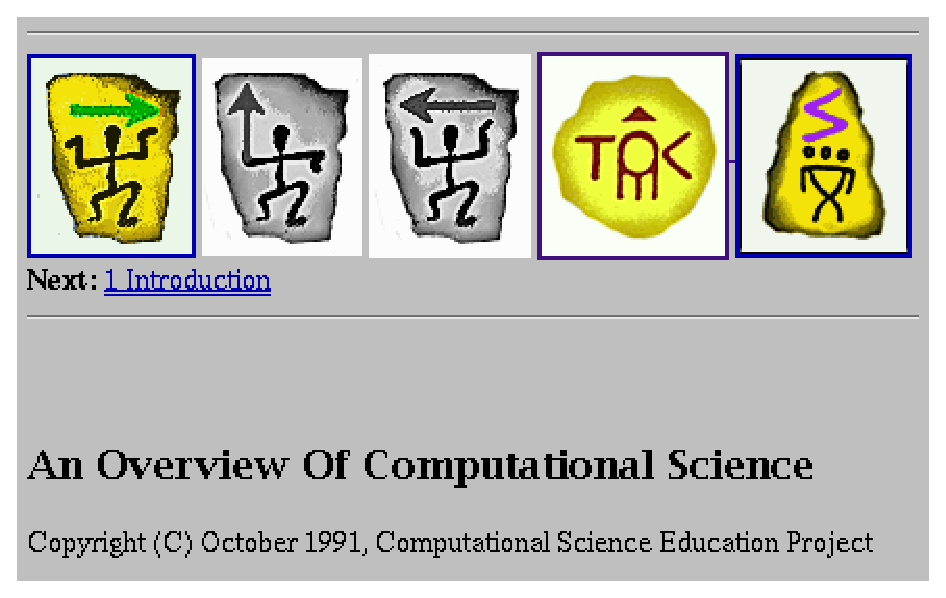
\includegraphics[width=5in]{psfiles/figure}
    \latex{\addtocounter{footnote}{-1}}
    \caption{A sample figure showing part of a page generated by
       \latextohtml{} containing a customised navigation panel 
       (from the 
        CSEP project).}\label{fig:example}
\end{figure}
\end{verbatim}
%begin{latexonly}
\end{small}
%end{latexonly}

\index{figures}%
\index{figure@\env{figure} environment}%
\index{environment!figure@\env{figure}}%
\index{Computer~Science~Education~Project!CSEP}% 
\begin{figure}[hbt]
    \htmlimage{thumbnail=0.5}
    \htmlborder{5}
    \centering 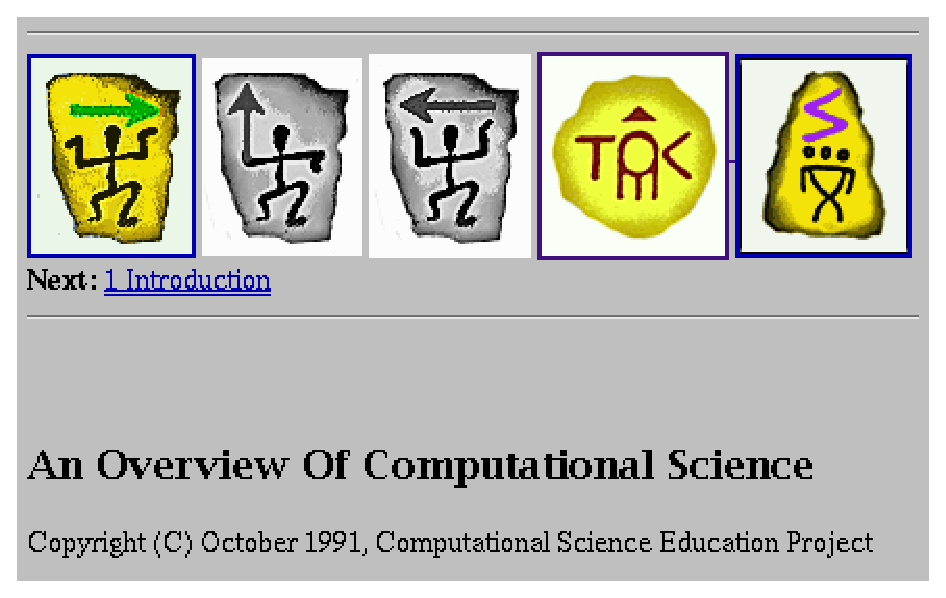
\includegraphics[width=5in]{psfiles/figure}
    \latex{\addtocounter{footnote}{-1}}%
    \caption{A sample figure showing part of a page generated by
       \protect\latextohtml{} containing a customised navigation panel 
       (from the 
        CSEP project).}\label{fig:example}
\end{figure}


\index{htmlimage@\Lc{htmlimage}!overrides configuration}%

\noindent
The \Lc{htmlimage} command is also often useful to cancel-out the
effect of the configuration variable \fn{\$FIGURE\_SCALE\_FACTOR}.
For example to avoid resizing a color screen snap despite 
the value of \fn{\$FIGURE\_SCALE\_FACTOR} it is possible to 
use \verb|\htmlimage{scale=0}|\,.


\subsubsection{Image Sharing and Recycling\label{recycling}}%
%\subsection{Image Sharing and Recycling\label{recycling}}%
\index{images!recycling}\index{images!sharing}%
It is not hard too see how reasonably sized papers,
especially scientific articles, can require
the use of many hundreds of external images.  For this reason,
image sharing and recycling is of critical importance.
In this context, ``sharing'' refers to the use of one
image in more than one place in an article.  ``Recycling''
refers to the use of an image left over from a previous
run of \latextohtml.  Without this ability, every instance of an
image would have to be regenerated each time even the
slightest change were made to the document.

\index{images!thumbnail}\index{thumbnail}%
\index{images!small images}%
\index{images!image-maps}%
\index{images!order-sensitive}%
\index{images!order-insensitive}%
\index{equations!array}%
\index{environment!\env{equation}}\index{environment!eqnarray@\env{eqnarray}}%
\index{eqnarray@\env{eqnarray} environment}\html{\\}%
%
All types of images can be shared.  These include ``small images''
and figures with or without \htmlref{thumbnails}{thumbnail}
and \htmlref{image-maps}{ImageMaps}.
Furthermore, most images can also be reused.  The only
exception are those which are \emph{order-sensitive},
meaning that their content depends upon their location.
Examples of order-sensitive images are \env{equation} 
and \env{eqnarray} environments, 
when \Cs{html\_version 2.0} has been specified;
this is because their figure numbers are part of the image.

\index{figures!captions}%
\index{tables!captions}\html{\\}%

Figures and tables with captions, on the other hand, 
are order-insensitive because the figure numbers 
are not part of the image itself.%
Similarly when \HTMLiii{} code is being produced, equation
numbers are no longer part of the image.
Instead they are placed in a separate cell of a \HTMLtag{TABLE}.
So most images of mathematical formulas can be reused also.%


\subsubsection{Quality of Printed Images\label{printqual}}
%\subsection{Quality of Printed Images\label{printqual}}
%
%% \begin{htmlonly}
Since it is often desirable to get a good quality print on paper
directly from the browser, \hyperref{here are}{Figure~}{ shows}{eq:pics15} 
the same equations as \hyperref[page]{earlier}{on page~}{}{eq:pics}.
This time the `\texttt{extrascale=}' option has been used with a value of 1.5\,.
More than twice the number of pixels are available, 
for a cost of approximately 1.7 times the disk-space\footnote{This figure
varies with the graphics format used, and the complexity of the actual image.}.

%% \end{htmlonly}

\begin{figure}[hb]
%% \begin{htmlonly}
%% \begin{makeimage}
%% \end{makeimage}
%% \begin{equation}
%% \htmlimage{no_antialias,extrascale=1.5}
%% \Phi_{l+1,m,n} = \Bigl(\Phi+h\frac{\partial\Phi}{\partial x} +
%% \frac{1}{2}h^2\frac{\partial^2\Phi}{\partial x^2} +
%% \frac{1}{6}h^3\frac{\partial^3\Phi}{\partial x^3} + \,\ldots\,\Bigr)_{l,m,n}
%% \end{equation}
%% \begin{eqnarray}
%% \htmlimage{extrascale=1.5}
%% \frac{\Phi_{l+1,m,n}-2\Phi_{l,m,n}+\Phi_{l-1,m,n}}{h^{2}} +
%% \frac{\Phi_{l,m+1,n}-2\Phi_{l,m,n}+\Phi_{l,m-1,n}}{h^{2}} \nonumber \\
%% + \frac{\Phi_{l,m,n+1}-2\Phi_{l,m,n}+\Phi_{l,m,n-1}}{h^{2}} = -I_{l,m,n}(v)
%% \end{eqnarray}
%% \end{htmlonly}
%% %
%% \begin{latexonly}
\begin{equation}
 \hbox{\scalebox{.4}{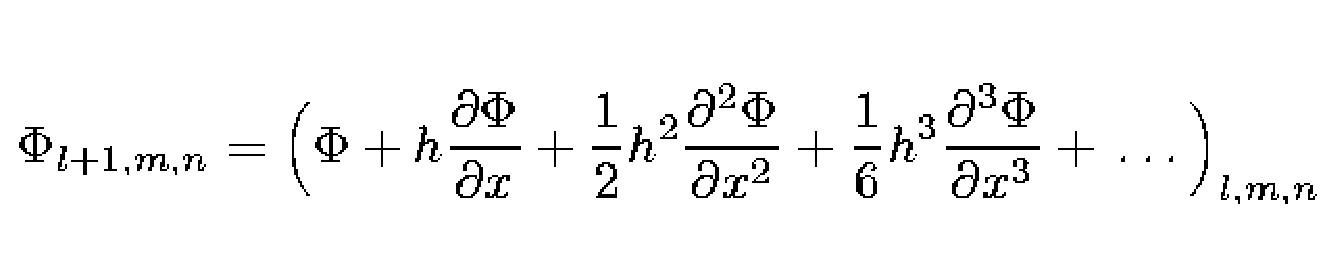
\includegraphics{psfiles/eqn15}}}
\end{equation}%
\begin{eqnarray}
 \nonumber
 \hbox{\scalebox{.4}{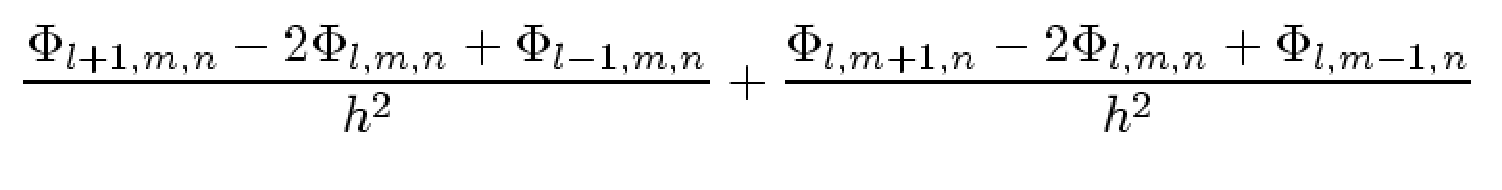
\includegraphics{psfiles/eqarrA15}}}
 &&\\
 \hbox{\scalebox{.4}{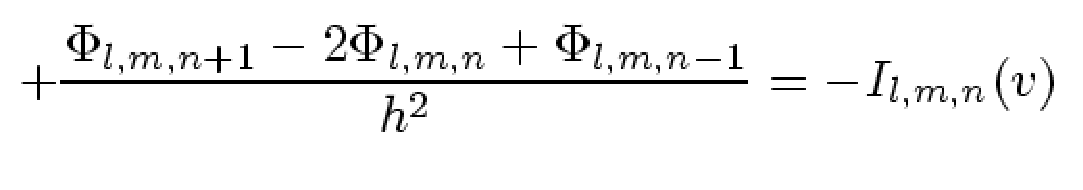
\includegraphics{psfiles/eqarrB15}}}
 &&
\end{eqnarray}
%% \end{latexonly}
\caption{Displayed math environments with \emph{extra-scale} of 1.5}
\label{eq:pics15}%
\end{figure}

%% \begin{latexonly}
\noindent
Since it is often desirable to get a good quality print on paper
directly from the browser, \hyperref{here are}{Figure~}{ shows}{eq:pics15}
the same equations as \hyperref[page]{earlier}{on page~}{}{eq:pics}.
This time the `\texttt{extrascale=1.5}' option has been used. This value of 1.5
means that more than twice the number of pixels are available,
for a cost of approximately 1.7 times the disk-space\footnote{This figure
varies with the graphics format used, and the complexity of the actual image.}.
%% \end{latexonly}
\noindent
On-screen these images appear slightly blurred or indistinct. 
However there can be marked improvement in the print quality,
when printed from some browsers; others may show no improvement at all. 
The ``anti-aliasing'' helps on-screen. In the printed version
jagged edges are indeed softened, but leave an overall fuzziness. 


\hyperref{Here are}{Figure~}{ shows}{eq:pics2} 
the same equations yet again; this time with `\texttt{extrascale=2.0}'.
Now there are 4~times the pixels at a cost of roughly 2.45~times the disk space.
Compared with the previous images (having 1.5~times extra-scaling), 
there is little difference in the on-screen images.
Printing at 300\,dpi shows only a marginal improvement;
but at 600\,dpi the results are most satisfying, especially when
scaled to be comparable with normal 10\,pt type\latex{, as here}.

\begin{figure}[ht]
%% \begin{htmlonly}
%% \begin{makeimage}
%% \end{makeimage}
%% \begin{equation}
%% \htmlimage{no_antialias,extrascale=2}
%% \Phi_{l+1,m,n} = \Bigl(\Phi+h\frac{\partial\Phi}{\partial x} +
%% \frac{1}{2}h^2\frac{\partial^2\Phi}{\partial x^2} +
%% \frac{1}{6}h^3\frac{\partial^3\Phi}{\partial x^3} + \,\ldots\,\Bigr)_{l,m,n}
%% \end{equation}
%% \begin{eqnarray}
%% \htmlimage{extrascale=2}
%% \frac{\Phi_{l+1,m,n}-2\Phi_{l,m,n}+\Phi_{l-1,m,n}}{h^{2}} +
%% \frac{\Phi_{l,m+1,n}-2\Phi_{l,m,n}+\Phi_{l,m-1,n}}{h^{2}} \nonumber \\
%% + \frac{\Phi_{l,m,n+1}-2\Phi_{l,m,n}+\Phi_{l,m,n-1}}{h^{2}} = -I_{l,m,n}(v)\;.
%% \end{eqnarray}
%% \end{htmlonly}
%% %
%% \begin{latexonly}
\begin{equation}
 \setbox1=\hbox{\scalebox{.3}{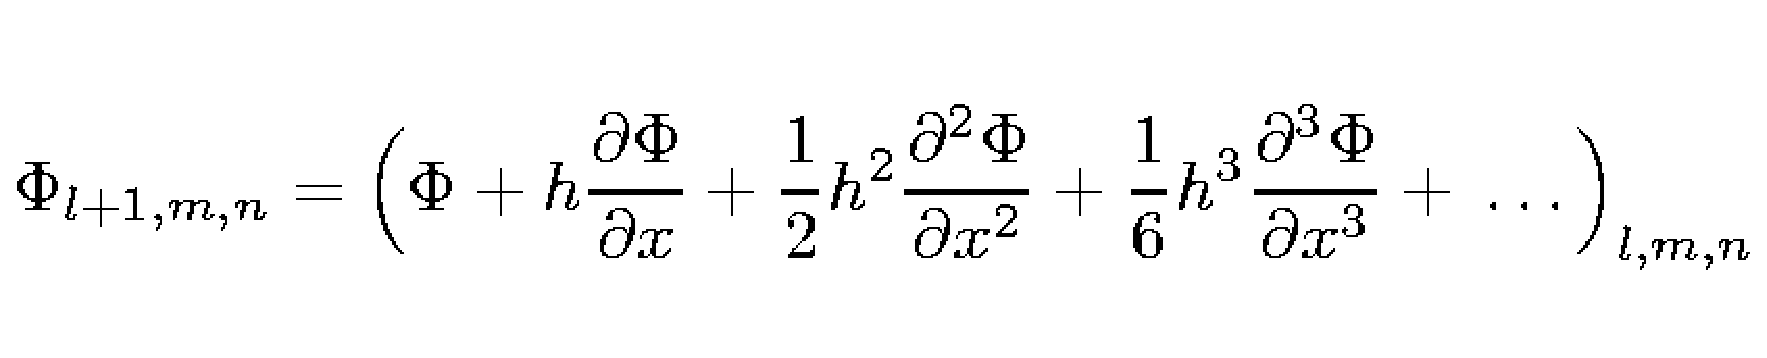
\includegraphics{psfiles/eqn2}}}
 \lower.5\ht1 \box1
\end{equation}
\begin{eqnarray}
 \nonumber
 \setbox1=\hbox{\scalebox{.3}{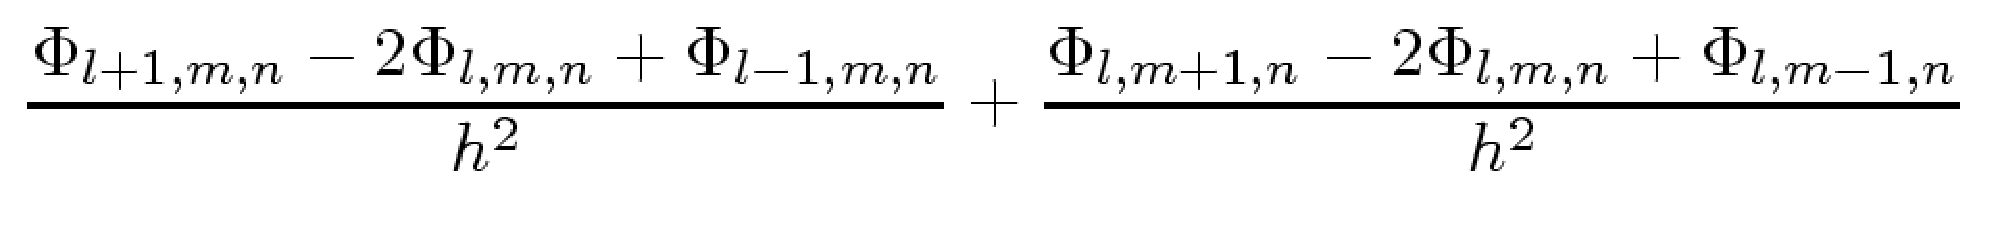
\includegraphics{psfiles/eqarrA2}}}
 \lower.5\ht1 \box1&&\\
 \setbox1=\hbox{\scalebox{.3}{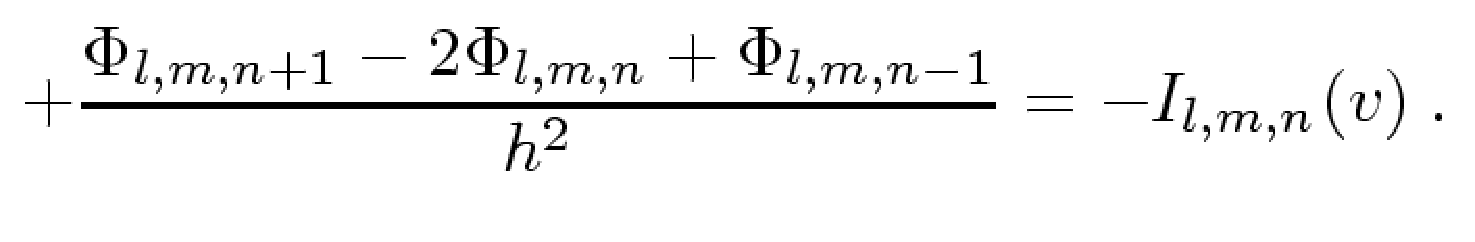
\includegraphics{psfiles/eqarrB2}}}
 \lower.5\ht1 \box1&&
\end{eqnarray}
%% \end{latexonly}
\caption{Displayed math environments with \emph{extra-scale} of 2.0}
\label{eq:pics2}
\end{figure}



\subsection{Figures, Tables and Arbitrary Images\label{sec:figs}}
%\section{Figures, Tables and Arbitrary Images\label{sec:figs}}
\index{tables}%
\index{environment!arbitrary}\index{arbitrary environments}\html{\\}% 
This section is to explain how the translator handles figures, tables
and other environments. 
Compare the paper with the online version.

When the common version of \texttt{HTML} was only 2.0, then almost all
complicated environments were represented using images. However with
\texttt{HTML} 3.2, there is scope for sensible layout of tables,
and proper facilities for associating a caption with a figure or table.
To take advantage of this, the \env{figure} environment now has its
contents placed within \HTMLtag{TABLE} tags; any caption is placed
as its \HTMLtag{CAPTION}.

For consistency with former practice, the contents of the \env{figure}
environment are usually represented by generating an image. 
This is frequently exactly what is required; but not always.
\hyperref[page]{In another section}{On page~}{}{makeimage} it is 
described how to use the \env{makeimage} environment,
defined in the \fn{html.sty} package, to determine just which parts (if any)
of a \env{figure} environment's contents should be made into images,
the remainder being treated as ordinary text, etc.

\medskip
\index{table@\env{table} environment}%
\index{environment!table@\env{table}}\html{\\}%
\paragraph*{\env{table} and \env{tabular} environments.}

Similarly the \env{makeimage} environment can be used within
a \env{table}, though usually this is used with a \env{tabular}
or other table-making environment, such as \env{tabbing} or
\env{longtable} or \env{supertabular}.
Here is a simple example, from the \LaTeX{} \htmlcite{`blue book'}{lamp:latex}.

\begin{table}[hbt]
\begin{center}
\begin{tabular}{||l|lr||}   \hline
gnats   &       gram    &       \$13.65  \\ \cline{2-3}
        &       each    &        .01    \\ \hline
gnu     &       stuffed &        92.50  
                \\  \cline{1-1} \cline{3-3}
emur    &               &       33.33   \\ \hline
armadillo       & frozen        &       8.99 \\ \hline
\end{tabular}
\caption{A sample table taken from \protect\cite{lamp:latex}%}
\index{table@\env{table} environment}%
\index{environment!table@\env{table}}}%
\label{tab}
\end{center}
\end{table}

\begin{htmlonly}
When using \texttt{ -html\_version 2.0} to get code compatible
with the \texttt{HTML} 2.0 standard, an image is made of the
table, as follows:
%
\begin{table}[ht]
\begin{center}
\begin{makeimage}
\begin{tabular}{||l|lr||}   \hline
gnats   &       gram    &       \$13.65  \\ \cline{2-3}
        &       each    &        .01    \\ \hline
gnu     &       stuffed &        92.50  
                \\  \cline{1-1} \cline{3-3}
emur    &               &       33.33   \\ \hline
armadillo       & frozen        &       8.99 \\ \hline
\end{tabular}
\end{makeimage}
\caption{Alternate view of the table from \protect\cite{lamp:latex}}
\label{tab:alt}
\end{center}
\end{table}
\end{htmlonly}
%
%begin{latexonly}
\noindent
Table~\ref{tab:alt} is a screen-shot of how the resulting table appears on-screen,
using a typical browser supporting \HTMLiii.
Here it is scaled down by 70\% to compensate for the 14\,pt fonts being used when
the screen-shot was taken.
%
\begin{table}[ht]
\begin{center}
 \scalebox{.7}{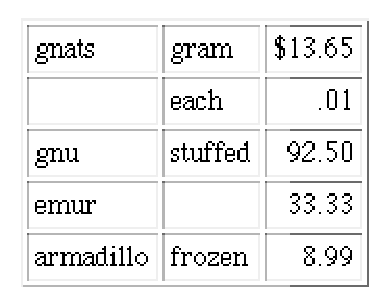
\includegraphics{psfiles/table}}
\caption{Alternate view of the table from \protect\cite{lamp:latex}}
\label{tab:alt}
\end{center}
\end{table}
%end{latexonly}

\medskip
\index{minipage@\env{minipage} environment}%
\index{environment!minipage@\env{minipage}}\html{\\}%
\paragraph*{\env{minipage} environments.}

The special feature of \env{minipage} environments is in the
way \Lc{footnote} and \Lc{footnotemark} commands are handled. 
These are numbered separately from the rest of the footnotes
throughout the document, and the notes themselves are collected together 
to be displayed at the end of the \env{minipage}'s contents.

\medskip
\begin{minipage}{.9\textwidth}
%begin{latexonly}
\renewcommand{\thempfootnote}{\alph{mpfootnote}}
%end{latexonly}
\begin{tabular}{|l|l|} \hline
\textbf{Variable} & \textbf{Meaning} \\ \hline
none      & none                   \\
Jacobi    & $m$-step Jacobi iteration\footnote[1]{one footnote} \\
SSOR      & $m$-step SSOR iteration\footnotemark[1] \\
IC        & Incomplete Cholesky factorization\footnote[2]{another footnote} \\
ILU       & Incomplete LU factorization\footnotemark[2] \\ \hline
\end{tabular}
\end{minipage}

\bigskip\noindent
The code used for this example was as follows\footnote{%
Thanks to John Turner \Email{turner@lanl.gov} for this example, 
which was used in developing
code to handle \env{minipage} environments correctly.}
%begin{latexonly}
\begin{small}
%end{latexonly}
\begin{verbatim}
\begin{minipage}{.9\textwidth}
\renewcommand{\thempfootnote}{\alph{mpfootnote}}
\begin{tabular}{|l|l|} \hline
\textbf{Variable} & \textbf{Meaning} \\ \hline
none      & none                   \\
Jacobi    & $m$-step Jacobi iteration\footnote[1]{one footnote} \\
SSOR      & $m$-step SSOR iteration\footnotemark[1] \\
IC        & Incomplete Cholesky factorization\footnote[2]{another footnote} \\
ILU       & Incomplete LU factorization\footnotemark[2] \\ \hline
\end{tabular}
\end{minipage}
\end{verbatim}
%begin{latexonly}
\end{small}
%end{latexonly}

\bigskip\noindent
\textbf{Warning: }
With some figures, especially when containing graphics imported using
\Lc{includegraphics} or other special macros, the background color
may come out as a shade of grey, rather than white or transparent.
This is due to a setting designed to enhance anti-aliasing of text
within images; e.g. for mathematics.
To alleviate this possible problem, the \Cs{white} command-line option
can be used, to ensure a white background for images of \env{figure}
environments. 
Alternatively, set the \fn{\$WHITE\_BACKGROUND} 
\hyperref{variable}{variable (see section }{)}{cs_white}.


\subsection{Document Classes and Options\label{sec:cls}}
\tableofchildlinks*
\index{document class}%
In general the standard \LaTeX{} document-classes: 
\texttt{article}, \texttt{report}, \texttt{book}, \texttt{letter}, \texttt{slides}
are translated by \latextohtml{} in the same way. 
Currently the only real difference is with the display of section-numbering,
when the \htmlref{\Cs{show\_section\_numbers}}{showsecnums} switch is used,
and when numbering of \htmlref{theorem-like environments}{theoremenvs} 
is linked to section-numbering.

\index{document class!loads file@loads a \texttt{.perl} file}%
\index{document class!options}%

These differences are achieved using a mechanism that automatically loads a file:
\fn{article.perl}, \fn{report.perl}, \fn{book.perl}, \fn{letter.perl}, \fn{slides.perl} 
according to the requested document-class. 
These files contain \Perl{} code and are located in the \fn{styles/} directory.
If a file of the same name exists in the working directory, this will be loaded
instead.

Typically such files \texttt{\Meta{class}.perl} contain code to define subroutines 
or sets values for variables that will affect how certain translations are performed. 
There can be code that is executed only when specific class-options are specified
along with the chosen document-class.
For example, the \fn{foils.perl} implementation of \FoilTeX's \env{foils} class
defines code create a new sub-section for each `foil'.
It also has code which allows \latextohtml{} to ignore those of \FoilTeX's special 
formatting commands that have no relevance when constructing an \texttt{HTML} page.

\medskip 
\index{document class!loads file}%
\index{class-option!loads file}%

Any options given on the \Lc{documentclass} or \Lc{documentstyle} line
may also cause a file containing \Perl{} code to be loaded. 
Such a file is named \texttt{\Meta{option}.perl} for the appropriate \Meta{option}.
When such a file exists, in the local directory or in the \fn{styles/} directory,
it typically contains \Perl{} code to define subroutines or set values for variables 
that will affect how certain translations are performed.
There can be code that is executed only for specific document-classes.

Since the files for class-options are loaded after those for the document-class,
it is possible for the \texttt{\Meta{option}.perl} file to contain code that overrides
settings made within the document-class file.

\medskip\index{class-option!specific file}%
If a file named \texttt{\Meta{class}\_\Meta{option}.perl} happens to exist for
a given combination of document-class \Meta{class} and class-option \Meta{option},
then this will be loaded. 
When such a file exists, reading and executing its contents is done,
rather than executing any \Meta{class}\_\Meta{option} specific information
that may be contained in  \texttt{\Meta{class}.perl} or \texttt{\Meta{option}.perl}~.

\medskip
Currently there are no special option or class-option files provided with 
the \latextohtml{} distribution. It is hoped that users will identify ways 
that specific features can be improved or adapted to specific classes of documents, 
and will write such files themselves, perhaps submitting them for general distribution.

\bigskip
\textbf{Note: }
This mechanism for handling code specific to different document classes
and class-options is more general than that employed by \LaTeXe.
New options can be defined for document-classes generally, or for specific classes,
without the need to have corresponding \texttt{.sty} or \texttt{.clo} files.
\LaTeX{} simply notes the existence of unusupported options---processing is not
interrupted.  



\subsection{Packages and Style-Files\label{sec:sty}}
%\section{Packages and Style-Files\label{sec:sty}}
\tableofchildlinks*
\index{support!for specific style-files}%
\index{support!for german language}\html{\\}%
%
Similar to the document-class mechanism described in
\hyperref{the previous section}{Section}{}{sec:cls},
\latextohtml{} provides a mechanism whereby the code to translate specific
packages and style-files is auto\-matic\-ally loaded, if such code is available.
For example, when use of a style such as \fn{german.sty} 
is detected in a \LaTeX{} source document, either by
\begin{itemize}
\item
a \Lc{usepackage} command of \LaTeXe;
\item
an option to the \Lc{documentstyle} command of \LaTeX\,2.09\,;
\item
an explicit \Lc{input} or \Lc{include} command;
\end{itemize}
the translator looks for a corresponding \texttt{.perl} file
having the same file-name prefix;
e.g. the file \fn{\$LATEX2HTMLDIR/styles/german.perl}.
If such a \texttt{.perl} file is found, 
then its code will be incorporated with the main script,
to be used as required. 

\index{extensions!examples}\html{\\}%

This mechanism helps to keep the core script smaller, as well as making
it easier for others to contribute and share solutions on  
how to translate specific style-files.
The current distribution includes the files to support the styles
listed in \hyperref{the table below}{Table~}{}{styles}.
These provide good examples of how you can create 
further extensions to \latextohtml.%

\index{style-files}\index{packages}%
%\begin{htmlonly}
%\begin{table}
%\end{htmlonly}
\begin{center}
%\begin{tabular}{|c|p{3in}|}
\begin{longtable}{|c|l|}
\caption{Supported \protect\latextohtml\ packages and style-files.}
\\\hline
\endhead
\hline
\endfoot
\label{styles}
\texttt{.perl}~file &\hfill\textbf{Description}\hfill\hfill~\\\hline
\env{\bf alltt}\index{environment!alltt@\env{alltt}}\index{alltt@\env{alltt} environment}%
 & Supports the \LaTeXe's \env{alltt} package.\label{alltt}\\
\env{\bf amsfonts}\index{package!AMSfonts@\env{amsfonts}}\index{AMS@\AmS-\LaTeX!amsfonts@\env{amsfonts} package}%
 & provides recognition of the special \AmS\ font symbols.\label{amsfonts}\\
\env{\bf amsmath}\index{package!AMSmath@\env{amsmath}}\index{AMS@\AmS-\LaTeX!amsmath@\env{amsmath} package}%
 & same as \fn{amstex.perl}.\label{amsmath}\\
\env{\bf amssymb}\index{package!AMSsymb@\env{amssymb}}\index{AMS@\AmS-\LaTeX!amssymb@\env{amssymb} package}%
 & same as \fn{amsfonts.perl}.\label{amssymb}\\
\env{\bf amstex}\index{package!AMStex@\env{amstex}}\index{AMS@\AmS-\LaTeX!amstex@\env{amstex} package}%
 & Supports much of the \AmS-\LaTeX{} package (not yet complete).\label{amstex}\\
\env{\bf babel}\index{package!babel@\env{babel}}\index{babel@\env{babel} package}%
 & Interface to \fn{german.perl} via the \env{babel} package.\label{babel}\\
\env{\bf changebar}\index{package!changebar@\env{changebar}}\index{changebar@\env{changebar} package}%
 & Provides rudimentary change-bar support.\label{changebar}\\
\env{\bf chemsym}\index{package!chemsym@\env{chemsym}}\index{chemsym@\env{chemsym} package}%
 & defines the standard atomic symbols.\label{chemsym}\\
\env{\bf color}\index{package!color@\env{color}}\index{color@\env{color} package}%
 & Causes colored text to be processed as ordinary text by \latextohtml.\label{color}\\
\env{\bf colordvi}\index{package!colordvi@\env{colordvi}}\index{color!colordvi@\env{colordvi} package}%
 & supports the Crayola colors.\label{crayola}\\
\env{\bf enumerate}\index{package!enumerate@\env{enumerate}}\index{enumerate@\env{enumerate} package}%
 & supports structured labels for \env{enumerate} environments.\label{enumerate}\\
\env{\bf epsbox}\index{package!epsbox@\env{epsbox}}\index{epsbox@\env{epsbox} package}%
 & Processes embedded figures not enclosed in a \env{figure} environment.\label{epsbox}\\
\env{\bf epsfig}\index{package!epsfig@\env{epsfig}}\index{epsfig@\env{epsfig} package}%
 & Processes embedded figures not enclosed in a \env{figure} environment.\label{epsfig}\\
\env{\bf finnish}\index{package!finnish@\env{finnish}}\index{finnish!finnish@\env{finnish} package}%
 & Support for the Finnish language.\label{finnish}\\
\env{\bf floatfig}\index{package!floatfig@\env{floatfig}}\index{floatfig@\env{floatfig} package}%
 & Processes floating figures.\label{floatfig}\\
\env{\bf floatflt}\index{package!floatflt@\env{floatflt}}\index{floatflt@\env{floatflt} package}%
 & Processes floating figures and tables.\label{floatflt}\\
\env{\bf foils}\index{class!foils@\env{foils}}\index{foils@\env{foils} class}\index{FoilTeX@\FoilTeX}%
 & Supports \FoilTeX{} system.\label{foils}\\
\env{\bf frames}\index{package!frames@\env{frames}}\index{frames@\env{frames} package}%
 & Provides separate frames for navigation and footnotes.\label{frames}\\
\env{\bf francais}\index{package!francais@\env{francais}}\index{french!francais@\env{francais} package}%
 & Support for the French language, same as \fn{french.perl}.\label{francais}\\
\env{\bf french}\index{package!french@\env{french}}\index{french@\env{french} package}%
 & Support for the French language.\label{french}\\
\env{\bf german}\index{package!german@\env{german}}\index{german@\env{german} package}%
 & Support for the German language.\label{german}\\
\env{\bf germanb}\index{package!germanb@\env{germanb}}\index{german!germanb@\env{germanb} package}%
 & Support for the German language, same as \fn{german.perl}.\label{germanb}\\
\env{\bf graphics}\index{package!graphics@\env{graphics}}\index{graphics@\env{graphics} package}%
 & Supports commands in the \env{graphics} package.\label{graphics}\\
\env{\bf graphicx}\index{package!graphicx@\env{graphicx}}\index{graphics!graphicx@\env{graphicx} package}%
 & Supports the alternate syntax of graphics commands.\label{graphicx}\\
\env{\bf harvard}\index{package!harvard@\env{harvard}}\index{citations!harvard@\env{harvard} package}%
 & Supports the \env{harvard} style of \htmlref{citation}{harvard} (same as fn{nharvard.perl}).\\
\env{\bf heqn}\index{package!heqn@\env{heqn}}\index{heqn@\env{heqn} package}%
 & Alters the way displayed equations are processed.\label{heqn}\\
\env{\bf hthtml}\index{environment!hthtml@\env{hthtml}}\index{hthtml@\env{hthtml} environment}%
 & gives an alternative syntax for specifying hyperlinks, etc.\label{hthtml}\\
\env{\bf htmllist}\index{environment!htmllist@\env{htmllist}}\index{htmllist@\env{htmllist} environment}%
 & Provides support for \htmlref{fancy lists}{htmllist}.\\
\env{\bf justify}\index{package!justify@\env{justify}}\index{justify@\env{justify} package}%
 & supports paragraph alignment---no longer needed.\\
\env{\bf latexsym}\index{package!latexsym@\env{latexsym}}\index{latexsym@\env{latexsym} package}%
 & supports the \LaTeX{} symbol font.\label{latexsym}\\
\env{\bf lgrind}\index{package!lgrind@\env{lgrind}}\index{lgrind@\env{lgrind} package}%
 & macros for nice layout of computer program code.\label{lgrind}\\
\env{\bf longtable}\index{package!longtable@\env{longtable}}%
\index{tables!longtable@longtable\env{longtable} package}%
 & supports use of long tables, as a single table.\label{longtable}\\
\env{\bf makeidx}\index{package!makeidx@\env{makeidx}}\index{makeidx@\env{makeidx} package}%
 & provides more sophisticated indexing.\label{makeidx}\\
\env{\bf multicol}\index{package!multicol@\env{multicol}}\index{columns!multicol@\env{multicol} package}%
 & suppresses requests for multi-columns.\label{multicol}\\
\env{\bf natbib}\index{package!natbib@\env{natbib}}\index{citations!natbib@\env{natbib} package}%
 & Supports many different styles for citations and bibliographies.\label{natbib}\\
\env{\bf nharvard}\index{package!nharvard@\env{nharvard}}\index{citations!nharvard@\env{nharvard} package}%
 & Supports harvard-style citations, using \env{natbib}.\label{nharvard}\\
\env{\bf seminar}\index{package!seminar@\env{seminar}}\index{seminar@\env{seminar} package}%
 & for creation of overhead-presentation slides.\label{seminar}\\
\env{\bf spanish}\index{package!spanish@\env{spanish}}\index{spanish@\env{spanish} package}%
 & Support for the Spanish language.\label{spanish}\\
\env{\bf supertabular}\index{package!supertabular@\env{supertabular}}\index{tables!supertabular@\env{supertabular} package}%
 & supports use super-tables, as an ordinary table.\label{supertabular}\\
\env{\bf texdefs}\index{package!texdefs@\env{texdefs}}\index{texdefs@\env{texdefs} package}%
 & Supports some raw \TeX{} commands.\label{texdefs}\\
\env{\bf verbatim}\index{package!verbatim@\env{verbatim}}\index{verbatim@\env{verbatim} package}%
 & Supports verbatim input of files.\label{verbatim}\\
\env{\bf verbatimfiles}\index{package!verbatimfiles@\env{verbatimfiles}}\index{verbatim!verbatimfiles@\env{verbatimfiles} package}%
 & Supports verbatim input of files, also with line-numbering.\label{verbatimfiles}\\
\env{\bf wrapfig}\index{package!wrapfig@\env{wrapfig}}\index{figures!wrapfig@\env{wrapfig} package}%
 & Supports wrapped figures.\label{wrapfig}\\
\env{\bf xspace}\index{package!xspace@\env{xspace}}\index{xspace@\env{xspace} package}%
 & Supports use of the \env{xspace} package and \Lc{xspace} command.\label{xspace}\\
\env{\bf xy}\index{package!xypic@\protect\Xy-pic}\index{xypic@\protect\Xy-pic package}%
\index{graphics!xy@\protect\Xy-pic package}%
 & Supports use of the \Xy-pic graphics package.\label{xypic}\\
%\hline
\end{longtable}
%\end{tabular}
\end{center}
%\begin{htmlonly}
%\end{table}
%\end{htmlonly}
%\end{table}
\index{extensions!require understanding@require understanding of \Perl{}}\html{\\}%
\noindent
The problem however, is that writing such extensions requires an understanding 
of \Perl{} programming and of the way the processing in \latextohtml{} is organised. 
Interfaces that are more ``user-friendly'' are being investigated.
Some of the techniques currently used are explained in 
\hyperref{a later section}{Section~}{}{sec:ext}.


\subsubsection{Fancy List-Markers\label{htmllist}}
%\subsection{Fancy List-Markers\label{htmllist}}
\index{htmllist@\env{htmllist} environment}%
\index{environment!htmllist@\env{htmllist}}%
%
An optional style-file \fn{htmllist.sty} has been provided which
produces fancier lists in the electronic version of the document%
\html{, }\htmlref{such as this}{listExample}.
This file defines a new \LaTeX{} environment \env{htmllist},
which causes a user-defined item-mark to be placed at each new
item of the list, and which causes the optional description
to be displayed in bold letters.
The filename prefix for the item-mark image can be given as an
optional parameter; see example below. The images distributed with
\latextohtml{} for this purpose are listed with the description
of the \verb|\htmlitemmark| command, which provides an alternative
means of choosing the item-mark, and allows the image to be changed
for different items in the list.

\index{htmlitemmark@\Lc{htmlitemmark}}%
\index{htmllist@\env{htmllist}!prints as@prints as \env{description}}%
\index{htmllist@\env{htmllist}!item-marks}%
\index{environment!htmllist@\env{htmllist}}\html{\\}%
%
The mark is determined
by the \verb|\htmlitemmark{|\Meta{item-mark}\verb|}| command.  
This command accepts either a mnemonic name for the \Meta{item-mark}, 
from a list of icons established at installation, or the URL of a mark
not in the installation list. 
The command \Lc{htmlitemmark} must be used \emph{inside} the 
\env{htmllist} environment in order to be effective, 
and it may be used more than once to change the mark within the list.  
The item-marks supplied with \latextohtml{} are 
\texttt{BlueBall}, \texttt{RedBall}, \texttt{OrangeBall}, \texttt{GreenBall}, 
\texttt{PinkBall}, \texttt{PurpleBall}, \texttt{WhiteBall} and \texttt{YellowBall}.
The \env{htmllist} environment is identical to 
the \env{description} environment in the printed version.

\index{htmllist@\env{htmllist}!example}%

\noindent 
An example of its usage is:
%begin{latexonly}
\begin{small}
%end{latexonly}
\begin{verbatim}
\begin{htmllist}[WhiteBall]
\item[Item 1:] This will have a white ball.
\item[Item 2:] This will also have a white ball.
\htmlitemmark{RedBall}%
\item[Item 3:] This will have a red ball.
\end{htmllist}
\end{verbatim}
%begin{latexonly}
\end{small}
%end{latexonly}

\noindent This will produce:\label{listExample}
\begin{htmllist}[WhiteBall]
%begin{latexonly}
\addtolength{\leftskip}{15pt}
%end{latexonly}
\item[Item 1:] This will have a white ball.
\item[Item 2:] This will also have a white ball.
\htmlitemmark{RedBall}%
\item[Item 3:] This will have a red ball.
\end{htmllist}

\index{floatfig@\env{floatingfigure} environment}%
\index{wrapfig@\env{wrapfigure} environment}%
\index{environment!floatingfigure@\env{floatingfigure}}%
\index{environment!wrapfigure@\env{wrapfigure}}\html{\\}%
\noindent
One can also obtain \LaTeXe\ style-files \fn{floatfig.sty} and 
\fn{wrapfig.sty}, which provide support for the \env{floatingfigure}
and \env{wrapfigure} environments, respectively.  These environments
allow text to wrap around a figure in the printed version, 
but are treated exactly as an ordinary \env{figure}s in the electronic version.  
They are described in \hypercite{The \LaTeX{} Companion}%
{\emph{The \LaTeX{} Companion}}{}{goossens:latex}.%

\subsubsection{Support for \FoilTeX\label{sec:foils}}
\index{foils@\env{foils} class}%
\index{FoilTeX@\FoilTeX} The \FoilTeX{} system presents some
additional problems for \latextohtml:
\begin{itemize}
\item It has additional commands like \Lc{foilhead} and
  \Lc{rotatefoilhead}, that roughly correspond to sectioning commands,
\item The images are produced at the sizes suitable for large screen
  presentation, but not for the HTML.
\end{itemize}
The package \fn{foils.perl} deals with these problems. It treats foils as
starred subsections and ignores \FoilTeX-specific commands that have no
meaning for HTML, like \Lc{LogoOn}. The header
\Lc{documentclass[}+\texttt{\it options}\verb+]{foils}+ in the
\fn{images.tex} file is substituted by the header
\Lc{documentclass[}\fn{\$FOILOPTIONS}\verb+]{+\fn{\$FOILCLASS}\verb+}+,
where the variables \fn{\$FOILOPTIONS} and \fn{\$FOILCLASS} can be set
in the configuration file (by default they are \texttt{'10pt'} and
\texttt{'article'} correspondingly).
A further variable \fn{\$FOILHEADLEVEL} holds the level of sectioning
at which a `foil' is to correspond; the default level is 4 (sub-section).

The \LaTeX{} style file \fn{foilhtml.sty} in the \fn{texinputs/}
directory provides some additional features for \FoilTeX{}. It implements
structural markup commands like \Lc{section},
\Lc{tableofcontents} for foils. See the directory \fn{docs/foilhtml/} for
the details.



\subsubsection{Indicating Differences between Document Versions\index{change-bars}}%
%\subsection{Indicating Differences between Document Versions\index{change-bars}}%
\latextohtml{} supports the \LaTeXe\ \fn{changebar.sty} package,
written by Johannes Braams \Email{JLBraams@cistron.nl}, for 
inserting \emph{change-bars} in a document in order to indicate 
differences from previous versions. This is a very primitive form of 
version control and there is much scope for improvement.

\index{change-bars!different versions}% 
Within the \LaTeX{} version of this manual two thicknesses of change-bar 
have been used. Thicker bars indicate changes introduced with version \textsc{v97.1}\,,
while thinner bars indicate earlier additions since \textsc{v96.1}\,.\html{\\}
Within the \texttt{HTML} version the change-bars clearly indicate the 
different revisions with explicit numbering.%
Within the \texttt{HTML} version, the graphic icons representing
the changebars can be followed by some text indicating the new version.
This is used repeatedly throughout\latex{ the online version of}
this manual. It is achieved using the command 
\verb|\cbversion{|\Meta{version}\verb|}|, immediately following
the \verb|\begin{changebar}|. 
This sets a variable \fn{\$cb\_version} to be used both at the beginning
and end of the environment. The value of this variable is retained,
to be used with other \env{changebar} environments, unless changed explicitly
by another occurrence of \fn{\$cb\_version}.

\smallskip\noindent
\textbf{Warning: }
\latextohtml{} will not correctly process \env{changebar} environments
that contain sectioning commands, even when the (sub)sections or
(sub)paragraphs are to occur on the same \texttt{HTML} page.
If this is required, use a separate \env{changebar} environment
within each (sub)section or (sub)paragraph.




\subsection{Indexing\label{index}\index{index|(}}%
%\section{Indexing\label{index}\index{index|(}}%
\index{index!section-names}%
\latextohtml{} automatically produces an Index consisting of the
arguments to all \Lc{index} commands encountered, if there are any.
A hyperlink is created to that point in the text where the 
\Lc{index} command occurred.

More sophisticated indexing is available by loading the \env{makeidx} package.
Most of the features described in \cite[Appendix~A]{lamp:latex} become available.
This includes:
%
\begin{htmllist}\htmlitemmark{RedBall}%
\index{index!styled entries}%
\item 
[styled entries, using `\texttt{@}' : ]
Entries of the form \verb|\index{|\Meta{sort-key}\verb|@|\Meta{styled-text}\verb|}|
produce \Meta{styled-text} as the entry, but sorted according to \Meta{sort-key}.

\index{index!hierarchical}%
\item 
[hierarchical entries, using `\texttt{!}' : ] 
Entries of the form
\verb|\index{|\Meta{item}\verb|!|\Meta{sub-item}\verb|}|
set the \Meta{sub-item} indented below the \Meta{item}.
Unlimited levels of hierarchy are possible, 
even though \LaTeX{} is limited to only 3 levels. 
The \Meta{sort-key}\verb|@|\Meta{styled-text} can be used at each level.

\index{index!page-ranges}%
\item 
[explicit ranges, using `\texttt{|(}' and `\texttt{|)}' : ]
This is perhaps more useful in the \LaTeX{} version. 
In the \texttt{HTML} version these simply insert words ``from'' and ``to'',
respectively, prior to the hyperlink to where the index-entry occurs.

\index{index!cross-link}%
\index{index!see@\texttt{\char124see}}%
\item 
[\texttt{|see\char123}\Meta{index-entry}\texttt{\char125} : ]
provides a textual reference to another indexed word or phrase, 
by inserting the word ``see''. 
This can be used in conjunction with \Lc{htmlref} to create a hyperlink
to the \Meta{index-entry}; viz.
\begin{verbatim}
\index{latexe@\LaTeXe |see{\htmlref{\LaTeX}{IIIlatex}}}
\end{verbatim}
where a \Lc{label} has been specified in some other index-entry, as follows:
\begin{verbatim}
\index{latex@\LaTeX\label{IIIlatex}}
\end{verbatim}

\index{index!emph@\texttt{\char124emph}}%
\item [\texttt{|emph} : ]
\strikeout{is recognised but \emph{ignored}; 
other \texttt{|\Meta{command}} commands are \emph{not} processed by \latextohtml{},
with the following exception\dots} is handled correctly, by applying
\Lc{emph} to the text of the generated hyperlink.

\index{index!style@\texttt{\char124}\Meta{style}}%
\item [\texttt{|}\Meta{style} : ]
where \Meta{style} is the name of \LaTeX{} style-changing command, 
without the initial `\Lc{}'; e.g. `\texttt{emph}', `\texttt{textbf}',
`\texttt{textit}', etc. The corresponding \LaTeX{} command is applied
to the text of the generated hyperlink.

\index{index!blank lines}%
\index{index!alphabetization}%
\item [blank lines and alphabetization: ]
Having precisely a single space-character after the \verb+|+ 
(e.g. \verb+\index{A| }+) 
places a blank line before the index entry and omits the hyperlink.
This is used mainly for visual formatting; it allows a break before the entries
starting with each letter, say. Using a printable-key, as in \verb+\index{Q@Q, R| }+,
is appropriate when there are no indexed words starting with `Q', say.

\index{index!quoted delimiters}%
\item [quoted delimiters: ]
The three special delimiters can be used within the printable portion,
if preceded by the double-quote character: \verb+"@+, \verb+"|+, \verb+"!+ 
and also \verb+""+ for the quote character itself. 
Also \verb|\"| produces an umlaut accent on the following character, 
when appropriate, else is ignored.
%
\end{htmllist}%

\index{index!cross-link}%
\index{index!labelled entries}\html{\\}\noindent
%
Furthermore, the printable part of an index entry can contain \texttt{HTML}
anchors; that is, hyperlinks and/or \verb|\label{...}|s.
This allows index entries to contain cross-links to other entries, for example,
as well as allowing index-entries to be the target of hyperlinks from elsewhere
within the document. 

The \htmlref{next section}{glossind} describes how this feature is used within this
manual to create a Glossary, containing a short description of all file-names,
configuration-variables and application software mentioned within the manual,
integrated with the Index. All occurrences of the technical names can be
easily found, starting from any other.

\index{index!labelled entries}

When a single item is indexed many times, it is sufficient 
to have a \Lc{label} command appearing within the printable portion 
of the first instance of an \verb|\index{...}| command for that item,
within a single document segment. 

\medskip

If the index-entries are in different segments of a segmented document, 
it is sufficient to have the  \verb|\index{...@...\label{...}}| appearing 
within that segment, in which the item is indexed, whose indexing information 
is loaded earliest via a \verb|\internal[index]{...}| command.
When in doubt, include one \verb|\index{...@...\label{...}}| per segment 
in which the item is indexed.

\index{index!cross-link}%
\index{index!cross-link incorrect}

For cross-links to work effectively within segmented documents,
the indexing command 
\verb|\index{...@...\label{...}}| \emph{must} occur earlier 
in the same segment than any use of 
\verb|\index{...@...\htmlref{...}{...}}| 
intended to create a link to that label. 
If the \Lc{label} occurs in a different segment,
then a \verb|\internal[index]{...}| command for that segment,
may be needed at the beginning of the segment with the \Lc{htmlref}\,.
When this is done incorrectly, the resulting link will be to the
segment where the indexed item occurred, 
rather than staying within the Index.

\htmlrule
\index{index!section-names}%
\index{index!cumbersome}%

\noindent
Since use of section-names, as the text for hyperlinks, can lead to a very long
and cumbersome Index, especially when single items have been indexed many times,
a further feature is provided to obtain a more compact Index.
 
\index{index!codified links}\html{\\}%
Use of the command-line option \Cs{short\_index} causes a codified 
representation of the sectioning to be used, rather than the full section-name.
The differences are as follows.
%
\begin{itemize}
%
\item
For example, `\texttt{2.1}' means sub-node~\#1 of node~\#2, 
viewing the entire document as a tree-like structure. 

\index{index!codified links!top-most node}%
\item
The top-most node is simply denoted `\verb|^|'.

\index{segmentation!child-links}%
\index{segmentation!codified index}%
\item
With a \htmlref{segmented document}{Segmentation}, 
each segment is codified separately 
using the \htmlref{\Meta{prefix}}{prefix} supplied for that segment.
The Index includes a legend of these prefixes, 
each giving the title of the leading page from the segment,
as a hyperlink to the place on that page where its 
child-links are displayed.

\index{index!codified links!for easier browsing}%
\item
Hyperlinks start on the same line as the index-key, 
rather than the next line, separated by `\texttt{|}'. 
This gives further compactification for easier browsing.

\index{index!with prefix@with \Meta{prefix}}%
\item
If \Cs{prefix \Meta{prefix}} has been specified, then the \Meta{prefix}
is prepended to the codified form. This is most useful for segmented documents. 
Now the top-most node is indicated by the bare \Meta{prefix}.
\end{itemize}
%
These features can also be obtained by setting the variable \fn{\$SHORT\_INDEX}
to have value `\texttt{1}', in a configuration or initialisation file;
provided, of course, that the document loads the \env{makeidx} package.%

\latex{\index{index|)}}



\subsubsection{Integrated Glossary and Index\label{glossind}}%
%\subsection{Integrated Glossary and Index\label{glossind}}%
\index{index!integrated with Glossary}%
\index{Glossary!integrated with Index}%

\noindent
A large number of different pieces of software are required to make
\latextohtml{} work effectively, as well as many files containing data or code 
to work with parts of this software. 
For this reason, a Glossary is included with this manual. 
It contains the names of all files, configuration variables, application software
and related technical terms, with a short description of what it is, or does,
and perhaps a URL for further reference. 

\index{Glossary!printed version}%
\index{Glossary!HTML@\texttt{HTML} version}\html{\\}%
In the printed version each item in the Glossary is accompanied by the page-numbers
on which the item is mentioned, somewhat like in the Index. 
For the \texttt{HTML} version, each glossary-item contains a hyperlink to an
index-entry, which then has links to each occurrence.
These extra index-entries do not appear in the printed version; 
indeed they also contain a hyperlink back to the corresponding glossary-entry. 

This feature is currently available only when using the \env{makeidx} package,
and needs also the \env{html} and \env{htmllist} packages.
It was developed for version 96.1f by Ross Moore,
incorporating an extensive revision of \fn{makeidx.perl}, as well as additions to
\latextohtml{} so that all aspects of indexing work correctly with segmented documents.

\bigskip
\noindent
Since \LaTeX{} provides no guidelines for how a Glossary should be constructed,
the technique used here will be explained in detail, for both the printed and
\texttt{HTML} versions. 

\begin{itemize}
\item
Firstly the \Lc{makeglossary} command, which is similar to \Lc{makeindex},
must appear in the document preamble, so that \LaTeX{} will record
uses of the \verb|\glossary{...}| command within a file \fn{manual.glo}.

This command is redundant in the \texttt{HTML} version, so is given a trivial
definition which is ignored by \LaTeX{}.\par

\item
Next, the words, phrases or technical terms to be included in the Glossary
are marked in the main text using the \Lc{glossary} command, used indirectly
via other macros. For example, file-names are inserted via 
\verb|\|\verb|fn{html.sty}|, \verb|\|\verb|fn{dvips}|,  \verb|\|\verb|appl{dvips}| etc. 
which both insert the text and create the glossary-entry; \textit{viz.}
%
%begin{latexonly}
\begin{small}
%end{latexonly}
\begin{verbatim}
\newcommand{\fn}[1]{\htmlref{\texttt{#1}}{GGG#1}\glossary{#1}}
\newcommand{\appl}[1]{\htmlref{\textsl{#1}}{GGG#1}%
  \Glossary{#1}{\textsl{#1}}}
\end{verbatim}
%begin{latexonly}
\end{small}
%end{latexonly}

\item
The expansions of \Lc{glossary}, and the slightly more general 
\Lc{Glossary}, are different for the printed and \texttt{HTML} versions.
For the \texttt{HTML} version the following definitions occur 
within an \env{htmlonly} environment:
%
%begin{latexonly}
\begin{small}
%end{latexonly}
\begin{verbatim}
\def\glossary#1{\index{#1@\texttt{#1} \label{III#1}%
  \htmlref{(G)}{GGG#1}}}
\def\Glossary#1#2{\index{#1@{#2} \label{III#1}\htmlref{(G)}{GGG#1}}}
\def\makeglossary{}
\end{verbatim}
%begin{latexonly}
\end{small}
%end{latexonly}
%
\dots while in \LaTeX{} we need only:\quad
\verb|\newcommand\Glossary[2]{\glossary{#1@#2}}|~.

Notice how the feature of \env{makeidx}, allowing the printable portion to
be separate from the sorting-key, is used to allow text-styles to be included within
both index-entries and glossary-entries. Indeed the purpose of \Lc{Glossary} is
to allow deviations from a fixed style, e.g. 
%
%begin{latexonly}
\begin{small}
%end{latexonly}
\begin{verbatim}
\newcommand{\MF}{\htmlref{\textsl{Metafont}}{GGGmetafont}%
  \Glossary{metafont}{\textsl{Metafont}}}%
\end{verbatim}
%begin{latexonly}
\end{small}
%end{latexonly}
%
Also notice that in the \texttt{HTML} version an index-entry is created that
includes, within its printable portion, both a \Lc{label} and a hyperlink.
The former, having name \texttt{III...}, will ultimately reside on the Index page, 
while the latter will point to an anchor named \texttt{GGG...} on the Glossary page.
These names must be distinct from any other names used with \Lc{label}s 
elsewhere in the document, hence the use of prefixes \texttt{III} and \texttt{GGG}.
A short string `\texttt{(G)}' is used for the text of the hyperlink in the Index.

\item
The text descriptions of the glossary-items are stored in a file 
called \fn{l2hfiles.dat}, with one description per line.
For the \texttt{HTML} version this file is actually read as input:
%
\begin{comment}
\begin{small}
\latex{\hskip15pt}\verb|\|\verb|begin{htmlonly}|%
\latex{\vskip-1.1\baselineskip\vskip-1.1\baselineskip\indentverb{15pt}}%
\begin{verbatim}
\section*{Glossary of variables and file-names\label{Glossary}}
\begin{htmllist}\htmlitemmark{OrangeBall}
\input l2hfiles.dat
\end{htmllist}
\end{verbatim}
\latex{\nobreak\vskip-1.1\baselineskip\nobreak\leavevmode\hskip15pt}%
\verb|\|\verb|end{htmlonly}|%
\end{small}%
\end{comment}
%
%begin{latexonly}
\begin{small}
%end{latexonly}
\begin{verbatim}
\section*{Glossary of variables and file-names\label{Glossary}}
\begin{htmllist}\htmlitemmark{OrangeBall}
  \input l2hfiles.dat
\end{htmllist}
\end{verbatim}
%begin{latexonly}
\end{small}%
%end{latexonly}

\noindent
For this reason alone it is desirable to have \fn{l2hfiles.dat} sorted alphabetically.\par

\item
The mechanism used for the \LaTeX{} version also requires the file to be sorted
strictly alphabetically, according to the sort-keys associated to each glossary entry.
\newline
(This requirement could be relaxed, but only with a loss in efficiency; see below.)

\LaTeX{} constructs its Glossary by running the \fn{makeindex} utility 
on the file \fn{manual.glo}, using the following command:
%
%begin{latexonly}
\begin{small}%
%end{latexonly}
\begin{verbatim}
makeindex -o manual.gls -s l2hglo.ist manual.glo
\end{verbatim}
%begin{latexonly}
\end{small}%
%end{latexonly}
%
Its output, which includes page numbering for an index, is stored in \fn{manual.gls}
and subsequently read by \LaTeX{} using:

%begin{latexonly}
\begin{small}%
%end{latexonly}
\begin{verbatim}
\InputIfFileExists{manual.gls}{\clearpage\typeout{^^Jcreating Glossary...}}
{\typeout{^^JNo Glossary, since  manual.gls  could not be found.^^J}}
\end{verbatim}%
%begin{latexonly}
\end{small}%
%end{latexonly}

\noindent
The configuration file \fn{l2hglo.ist} is included along with this manual.
It contains a portion that inserts tricky \TeX{} code at the beginning of \fn{manual.gls}.
This code extracts from \fn{l2hfiles.dat} that line corresponding to each glossary entry, 
then typesets it itemized within an environment called \env{theglossary}.

%begin{latexonly}
\begin{small}%
%end{latexonly}
\begin{verbatim}
\newenvironment{theglossary}{\begin{list}{}{%
  \setlength{\labelwidth}{20pt}%
  \setlength{\leftmargin}{\labelwidth}%
  \setlength\itemindent{-\labelwidth}%
  \setlength\itemsep{0pt}\setlength\parsep{0pt}%
  \rmfamily}}{\end{list}}
\end{verbatim}
%begin{latexonly}
\end{small}%
%end{latexonly}
%
Currently searching within \fn{l2hfiles.dat} is only done sequentially, stopping
at the end of the file. If an entry is not found then it is skipped and a message
printed to the log; the next entry will search from the top of the file.
If all entries are included and maintained in strict order, there will be no skipping 
and each line of \fn{l2hfiles.dat} is read exactly once.\par

\item
Within \fn{l2hfiles.dat} the data lines look like:
%
%begin{latexonly}
\begin{small}%
%end{latexonly}
\begin{verbatim}
\item[\gn{french.perl}] adds \Perl{} code to be compatible with the ...
\item[\gn{\textsl  {ftp}}] `File Transfer Protocols', network ...
\item[\gn{german.perl}] adds \Perl{} code to be compatible with the ...
...
\end{verbatim}
%begin{latexonly}
\end{small}%
%end{latexonly}
%
For the \LaTeX{} version the \verb|\item[\gn{...}]| is only used for pattern-matching, 
to find the correct data entry.
All typesetting is controlled from within \fn{manual.gls}.

However the \texttt{HTML} version requires the following definition:
%
%begin{latexonly}
\begin{small}%
%end{latexonly}
\begin{verbatim}
\newcommand{\gn}[1]{\texttt{#1}\label{GGG#1}\htmlref{\^}{III#1}}%  
\end{verbatim}
%begin{latexonly}
\end{small}%
%end{latexonly}
%
which establishes the hyperlink to the Index, marked by `\verb|^|', 
and provides the \Lc{label} to create the target in the Glossary 
for any \verb|\glossary{...}| command having the corresponding argument.%
\end{itemize}
